\section{Early Fire Detection Based on Aerial 360-Degree Sensors,
Deep Convolution Neural Networks and Exploitation of Fire Dynamic Textures}

%1
\begin{frame}
    \frametitle{\textit{Early Fire Detection Based on Aerial 360-Degree Sensors,
    Deep Convolution Neural Networks and Exploitation of Fire Dynamic Textures}}

    \Large 
    A multi-stages objection detection method is proposed, using:
    \normalsize
    \begin{itemize}
        \item \textbf{360-degree unlimited view image}
        \item \textbf{a novel post-validation adaptive method }
        \item \textbf{DeepLab V3+ model}
    \end{itemize}

    \begin{figure}[H]
        \centering
        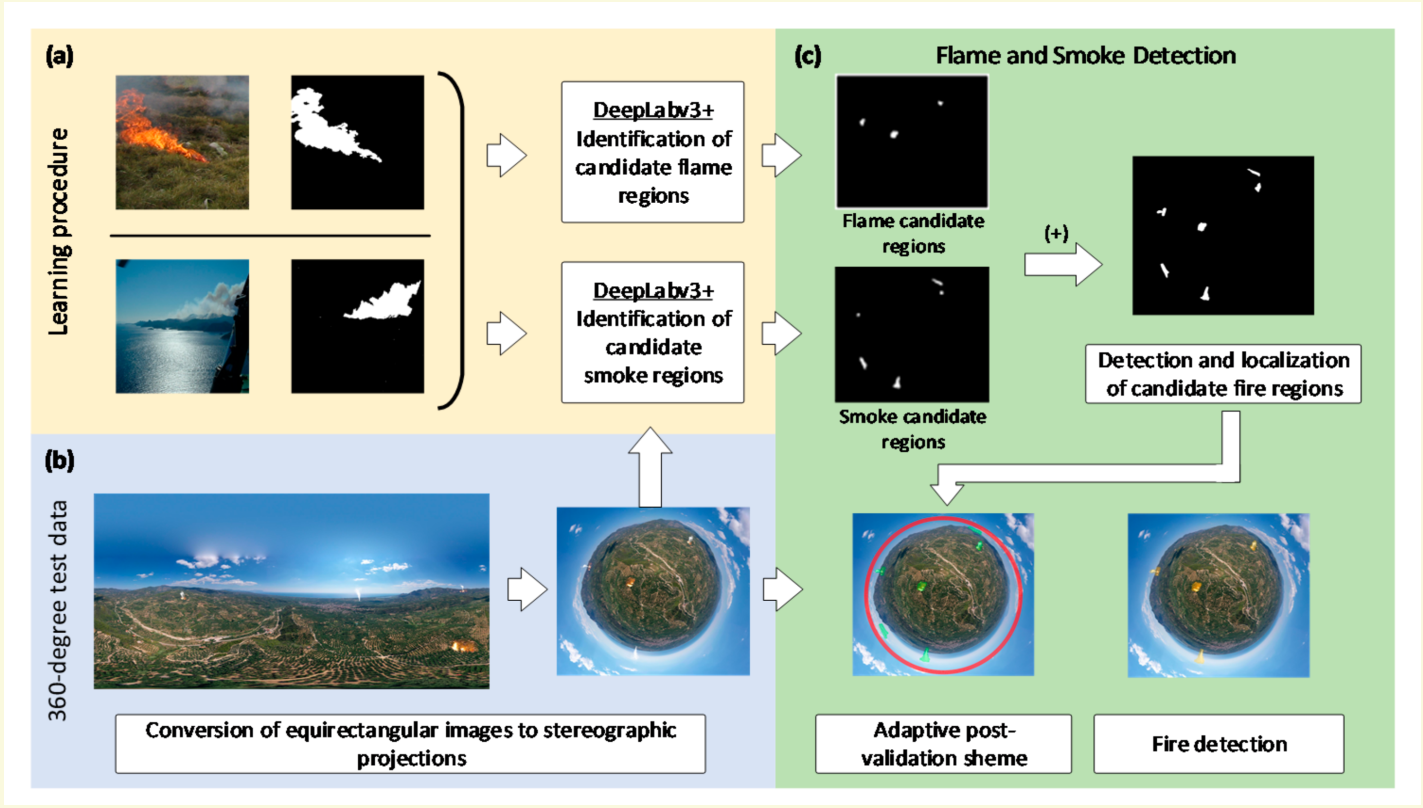
\includegraphics[width=0.7\textwidth]{./imgs/proposed_process}
    \end{figure}

\end{frame}

%2
\begin{frame}
    \frametitle{\textit{Early Fire Detection Based on Aerial 360-Degree Sensors
    ...  ~------~ Highlights}}

    \begin{itemize}
        \item \Large \colorbox{orange}{The 360-degree image:}\linebreak
            \normalsize
            Omnidirectional cameras can cover a wider field with only a single
            camera. Use the stereographic projection to map 3D to 2D.
        \item \Large \colorbox{orange}{The adaptive post-validation:}\linebreak
            \normalsize
            Use the KNN to cluster the cloud and the smoke around the horizon.
    \end{itemize}

    \begin{figure}[H]
        \centering
        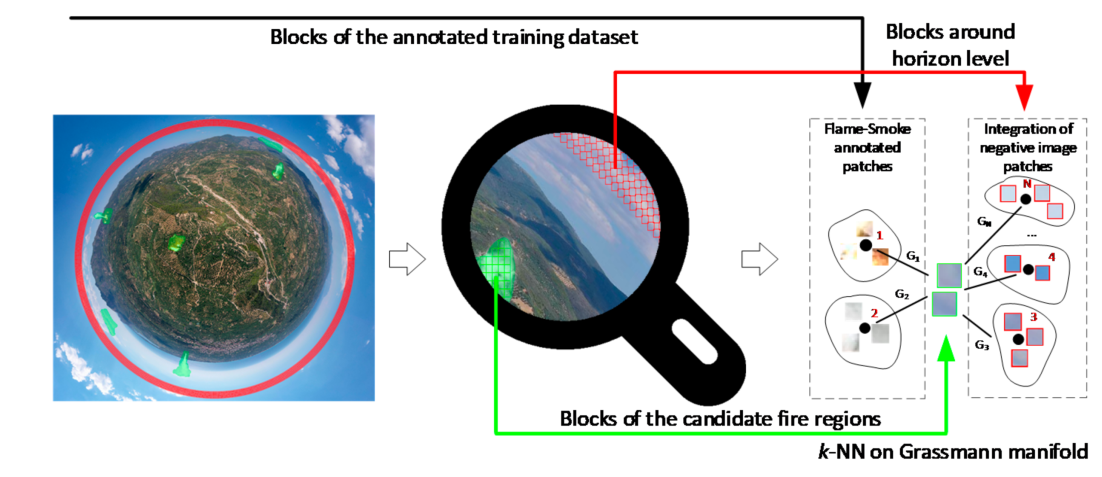
\includegraphics[width=0.7\textwidth]{./imgs/adaptive_validation}
    \end{figure}

\end{frame}
